\subsection{Demonstração Direta}

\begin{frame}[t]
\vskip 3cm
\begin{center}
{\Huge Demonstração Direta\\(ou natural)}
\end{center}
\end{frame}


\begin{frame}[t]{Idéia de uma prova lógica:}

\begin{figure}[!ht]
\centering 
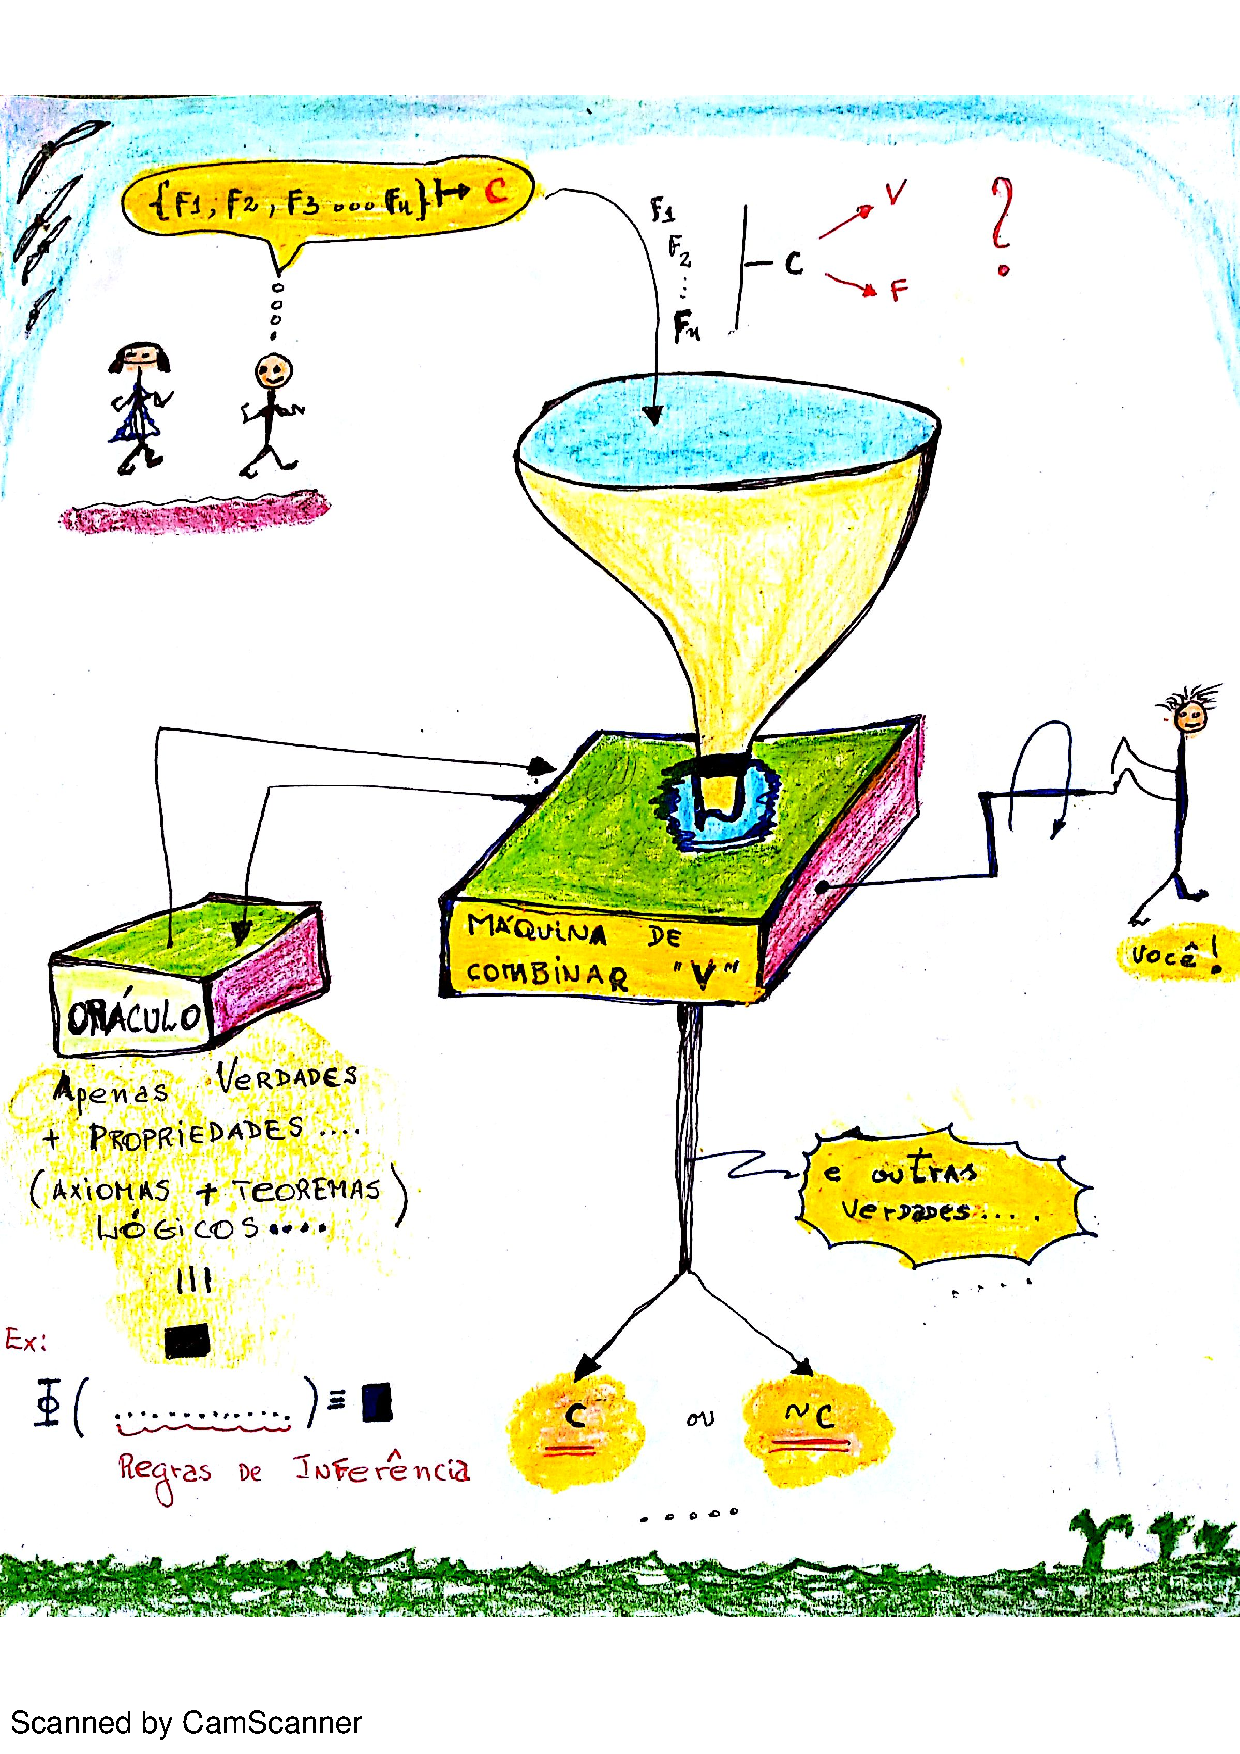
\includegraphics[width=0.65\textwidth, height=0.89\textheight]{provador_ilustrado.pdf}
%\caption{Ilustrando o conceito de provas -- explicação em aula}
%\label{fig_-system-architecture}
\end{figure}
\end{frame}


\begin{frame}[t]{Algo mais formal:}

\begin{figure}[!htb]
\centering 
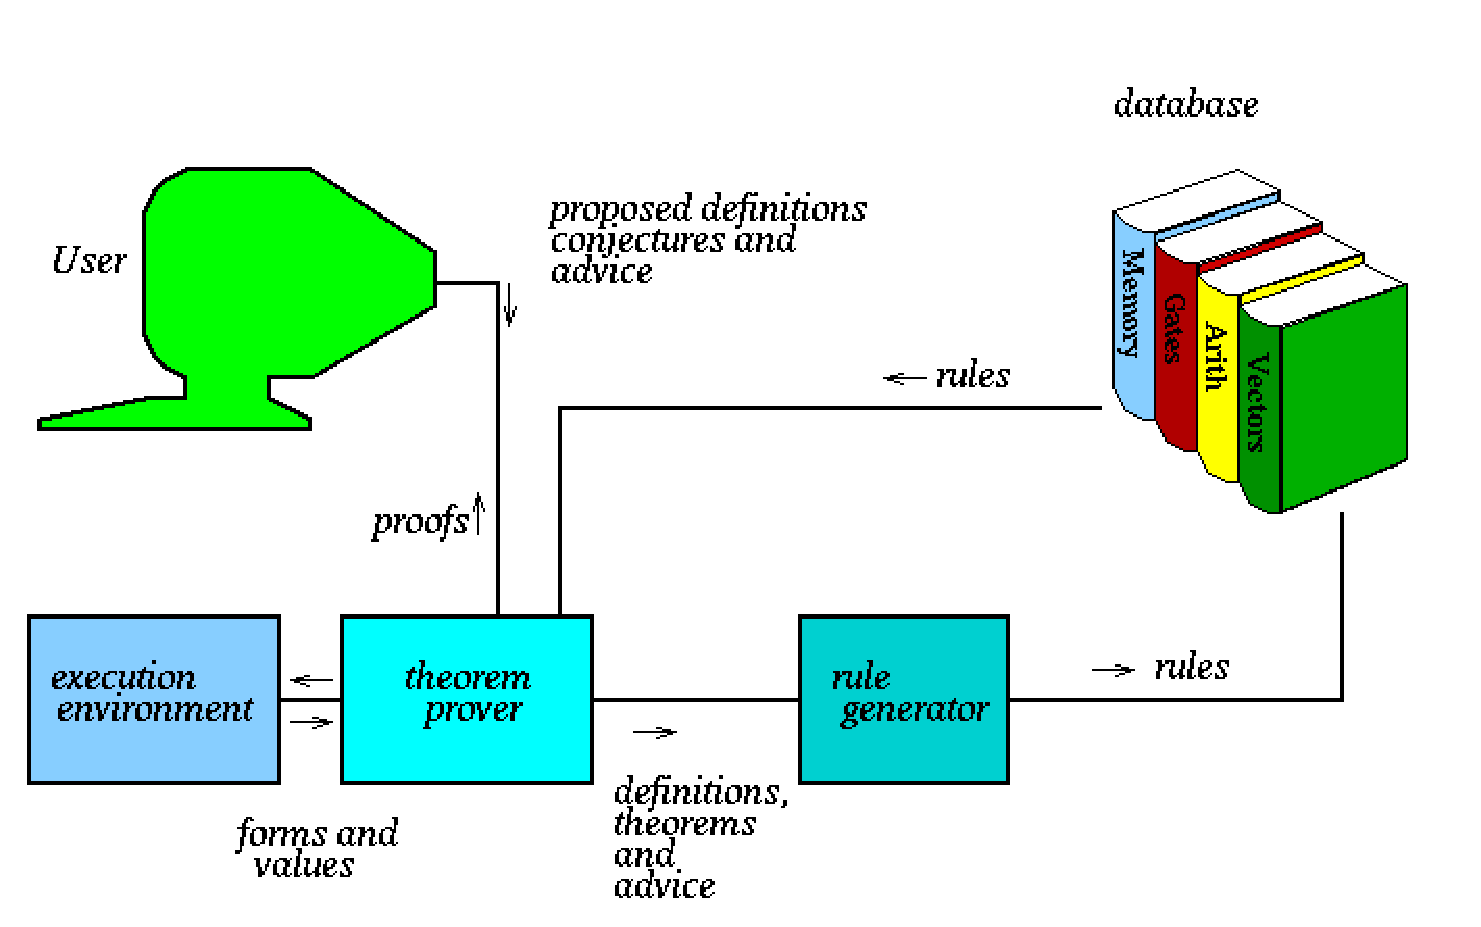
\includegraphics[width=0.8\textwidth, height=0.56\textheight]{proofer-system-architecture.pdf}
\caption{Ilustrando o conceito de provas -- explicação em aula}
\label{fig_-system-architecture}
\end{figure}
\end{frame}






\begin{frame}[t]{Demonstração Direta - Argumentos}
	\begin{itemize}
	\item Dadas as proposições ({\em premissas}) $p_1, p_2, \ldots, p_n$ e uma conclusão $q$, denota-se que: $$\{p_1, p_2, \ldots, p_n \} \vdash q$$
	
	\item {\bf Validade de Argumento:} um argumento é considerado válido se 
	$$p_1 \wedge p_2 \wedge \ldots \wedge p_n \Rightarrow q $$
	
	\item Assim a interpretação de um argumento válido (ver definição de $\Rightarrow$) é dado por: 
		$$\Phi^{n+1} ((p_1 \wedge p_2 \wedge \ldots \wedge p_n) \rightarrow q) \equiv \blacksquare$$
	
	\item Logo, esta é a definição de \textbf{teorema lógico} ou argumento válido: \underline{uma verdade}!
	
	\item Exemplo: $p \vdash p \vee q$ é sempre válido (um teorema!)
	
 \item Assim: $\Phi (p  \rightarrow ( p \vee q)) \equiv \blacksquare $
\end{itemize}
\end{frame}



\begin{frame}[t]{Demonstração Direta - Argumentos}
	Argumentos Válidos Fundamentais

	\begin{description}
	\item [Adição (AD)] $p \vdash p \vee q$
	
	\item [Simplificação (SIMP)] $\begin{array}{l}p \wedge q \vdash p\\p \wedge q \vdash q\end{array}$ 
	
	\item [Conjunção (CONJ)] $p, q \vdash p \wedge q$

	\item [Absorção (ABS)] $p \rightarrow q \vdash p \rightarrow(p \wedge q)$

	\item [Modus Ponens (MP)] $p \rightarrow q, p \vdash q$
	
	\item [Modus Tollens (MT)] $p \rightarrow q, \sim q \vdash \sim p$
	\end{description}
\end{frame}


\begin{frame}[t]{Demonstração Direta - Argumentos}
	Argumentos Válidos Fundamentais

	\begin{description}
	\item [Silogismo Disjuntivo (SD)] $\begin{array}{l}p \vee q, \sim p \vdash q\\p \vee q, \sim q \vdash p\end{array}$ 
	
	\item [Silogismo Hipotético (SH)] $p \rightarrow q, q \rightarrow r \vdash p \rightarrow r$ 

	\item [Dilema Construtivo (DC)] $p \rightarrow q, r \rightarrow s, p \vee r \vdash q \vee s$
	
	\item [Dilema Destrutivo (DD)] $p \rightarrow q, r \rightarrow s, \sim q \vee \sim s \vdash \sim p \vee \sim r$	
	\end{description}	
\end{frame}


\begin{frame}[t]{Demonstração Direta - Argumentos}

	\begin{description}
	\item[Regras de Inferência] ~~ 
	\begin{itemize}
	\item Escreve-se as premissas (em coluna), um traço horizontal e então escreve-se a conclusão
	\item Exemplo para a regra Modus Ponens (MP)	
	\end{itemize}	
	
	\vskip 1.5cm
	
	\begin{minipage}{0.3\textwidth}
	$	\begin{array}{l}
	p \rightarrow q  \\
	p  \\
	\hline
	q 
	\end{array}$
	\end{minipage}
	\begin{minipage}{0.3\textwidth}
	$	\begin{array}{l}
	\sim p \vee r \rightarrow s \wedge \sim q \\
	\sim p \vee r \\
	\hline
	s \wedge \sim q
	\end{array}$
	\end{minipage}
	\end{description}		
	
\end{frame}

\begin{frame}[t]{Validade mediante Regras de Inferência}

\begin{figure}[!htb]
\centering 
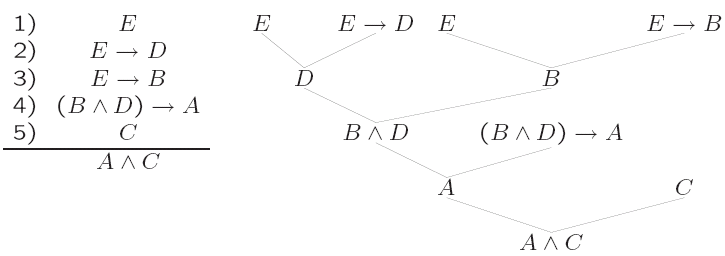
\includegraphics[width=0.8\textwidth, height=0.56\textheight]{example_proof.png}
\caption{Exemplo de prova simples -- explicação em aula}
\label{fig_arvore_prova_simples}
\end{figure}
\end{frame}


\begin{frame}[t]{Validade mediante Regras de Inferência}

	Verifique a validade para $p \rightarrow q, p \wedge r \vdash q$
	
\end{frame}

\begin{frame}[t]{Validade mediante Regras de Inferência}

	Verifique a validade para $p \rightarrow q, p \wedge r \vdash q$
	
	\vskip 1.5cm
	
	\begin{minipage}{0.5\textwidth}
	$	\begin{array}{ll}
	p \wedge r  & \\
	\hline
	p & \mathbf{por~(SIMP)}
	\end{array}$
	\end{minipage}
\end{frame}


\begin{frame}[t]{Validade mediante Regras de Inferência}

	Verifique a validade para $p \rightarrow q, p \wedge r \vdash q$
	
	\vskip 1.5cm
	
	\begin{minipage}{0.5\textwidth}
	$	\begin{array}{ll}
	p \wedge r  & \\
	\hline
	p & \mathbf{por~(SIMP)}
	\end{array}$
	\end{minipage}
	\begin{minipage}{0.3\textwidth}
	$	\begin{array}{ll}
	p \rightarrow q & \\
	p &  \\
	\hline
	q & \mathbf{por~(MP)}
	\end{array}$
	\end{minipage}
\end{frame}

\begin{frame}[t]{Validade mediante Regras de Inferência}

	Verifique a validade para $p \wedge q, p \vee r \rightarrow s \vdash p \wedge s$
	
\end{frame}

\begin{frame}[t]{Validade mediante Regras de Inferência}

	Verifique a validade para $p \wedge q, p \vee r \rightarrow s \vdash p \wedge s$
	
	\vskip 1.5cm
	
	$$\begin{array}{lll}
	(1) & p \wedge q  & \\
	(2) & p \vee r \rightarrow s & \\
	\hline
	\end{array}$$	
\end{frame}

\begin{frame}[t]{Validade mediante Regras de Inferência}

	Verifique a validade para $p \wedge q, p \vee r \rightarrow s \vdash p \wedge s$
	
	\vskip 1.5cm
	
	$$\begin{array}{lll}
	(1) & p \wedge q  & \\
	(2) & p \vee r \rightarrow s & \\
	\hline
	(3) & p & \mathbf{(1)~por~(SIMP)} \\
	\end{array}$$	
\end{frame}

\begin{frame}[t]{Validade mediante Regras de Inferência}

	Verifique a validade para $p \wedge q, p \vee r \rightarrow s \vdash p \wedge s$
	
	\vskip 1.5cm
	
	$$\begin{array}{lll}
	(1) & p \wedge q  & \\
	(2) & p \vee r \rightarrow s & \\
	\hline
	(3) & p & \mathbf{(1)~por~(SIMP)} \\
	(4) & p \vee r & \mathbf{(3)~por~(AD)} \\
	\end{array}$$	
\end{frame}

\begin{frame}[t]{Validade mediante Regras de Inferência}

	Verifique a validade para $p \wedge q, p \vee r \rightarrow s \vdash p \wedge s$
	
	\vskip 1.5cm
	
	$$\begin{array}{lll}
	(1) & p \wedge q  & \\
	(2) & p \vee r \rightarrow s & \\
	\hline
	(3) & p & \mathbf{(1)~por~(SIMP)} \\
	(4) & p \vee r & \mathbf{(3)~por~(AD)} \\
	(5) & s & \mathbf{(2,4)~por~(MP)} \\
	\end{array}$$	
\end{frame}


\begin{frame}[t]{Validade mediante Regras de Inferência}

	Verifique a validade para $p \rightarrow (q \rightarrow r), p \rightarrow q, p \vdash r$
	
	\vskip 1.5cm
	
	$$\begin{array}{lll}
	(1) & p \rightarrow (q \rightarrow r)  & \\
	(2) & p \rightarrow q & \\
	(3) & p & \\
	\hline
	\end{array}$$	
\end{frame}


\begin{frame}[t]{Validade mediante Regras de Inferência}

	Verifique a validade para $p \rightarrow (q \rightarrow r), p \rightarrow q, p \vdash r$
	
	\vskip 1.5cm
	
	$$\begin{array}{lll}
	(1) & p \rightarrow (q \rightarrow r)  & \\
	(2) & p \rightarrow q & \\
	(3) & p & \\
	\hline
	(4) & q \rightarrow r & \mathbf{(1,3) ~por~ (MP)}
	\end{array}$$	
\end{frame}


\begin{frame}[t]{Validade mediante Regras de Inferência}

	Verifique a validade para $p \rightarrow (q \rightarrow r), p \rightarrow q, p \vdash r$
	
	\vskip 1.5cm
	
	$$\begin{array}{lll}
	(1) & p \rightarrow (q \rightarrow r)  & \\
	(2) & p \rightarrow q & \\
	(3) & p & \\
	\hline
	(4) & q \rightarrow r & \mathbf{(1,3)~por~(MP)} \\
	(5) & q & \mathbf{(2,3)~por~(MP)}
	\end{array}$$	
\end{frame}


\begin{frame}[t]{Validade mediante Regras de Inferência}

	Verifique a validade para $p \rightarrow (q \rightarrow r), p \rightarrow q, p \vdash r$
	
	\vskip 1.5cm
	
	$$\begin{array}{lll}
	(1) & p \rightarrow (q \rightarrow r)  & \\
	(2) & p \rightarrow q & \\
	(3) & p & \\
	\hline
	(4) & q \rightarrow r & \mathbf{(1,3)~por~(MP)} \\
	(5) & q & \mathbf{(2,3)~por~(MP)} \\
	(6) & r & \mathbf{(4,5)~por~(MP)}
	\end{array}$$	
\end{frame}


\begin{frame}[t]{Validade mediante Regras de Inferência}

	Verifique a validade para $p \rightarrow q, p \wedge q \rightarrow r, \sim (p \wedge r) \vdash \sim p$
	
	\vskip 1.5cm
	
	$$\begin{array}{lll}
	(1) & p \rightarrow q  & \\
	(2) & p \wedge q \rightarrow r & \\
	(3) & \sim (p \wedge r) & \\
	\hline
	\end{array}$$	
\end{frame}


\begin{frame}[t]{Validade mediante Regras de Inferência}

	Verifique a validade para $p \rightarrow q, p \wedge q \rightarrow r, \sim (p \wedge r) \vdash \sim p$
	
	\vskip 1.5cm
	
	$$\begin{array}{lll}
	(1) & p \rightarrow q  & \\
	(2) & p \wedge q \rightarrow r & \\
	(3) & \sim (p \wedge r) & \\
	\hline
	(4) & p \rightarrow p \wedge q & \mathbf{(1)~por~(ABS)}
	\end{array}$$	
\end{frame}


\begin{frame}[t]{Validade mediante Regras de Inferência}

	Verifique a validade para $p \rightarrow q, p \wedge q \rightarrow r, \sim (p \wedge r) \vdash \sim p$
	
	\vskip 1.5cm
	
	$$\begin{array}{lll}
	(1) & p \rightarrow q  & \\
	(2) & p \wedge q \rightarrow r & \\
	(3) & \sim (p \wedge r) & \\
	\hline
	(4) & p \rightarrow p \wedge q & \mathbf{(1)~por~(ABS)} \\
	(5) & p \rightarrow r & \mathbf{(2,4)~por~(SH)}
	\end{array}$$	
\end{frame}


\begin{frame}[t]{Validade mediante Regras de Inferência}

	Verifique a validade para $p \rightarrow q, p \wedge q \rightarrow r, \sim (p \wedge r) \vdash \sim p$
	
	\vskip 1.5cm
	
	$$\begin{array}{lll}
	(1) & p \rightarrow q  & \\
	(2) & p \wedge q \rightarrow r & \\
	(3) & \sim (p \wedge r) & \\
	\hline
	(4) & p \rightarrow p \wedge q & \mathbf{(1)~por~(ABS)} \\
	(5) & p \rightarrow r & \mathbf{(2,4)~por~(SH)} \\
	(6) & p \rightarrow p \wedge r & \mathbf{(5)~por~(ABS)}
	\end{array}$$	
\end{frame}


\begin{frame}[t]{Validade mediante Regras de Inferência}

	Verifique a validade para $p \rightarrow q, p \wedge q \rightarrow r, \sim (p \wedge r) \vdash \sim p$
	
	\vskip 1.5cm
	
	$$\begin{array}{lll}
	(1) & p \rightarrow q  & \\
	(2) & p \wedge q \rightarrow r & \\
	(3) & \sim (p \wedge r) & \\
	\hline
	(4) & p \rightarrow p \wedge q & \mathbf{(1)~por~(ABS)} \\
	(5) & p \rightarrow r & \mathbf{(2,4)~por~(SH)} \\
	(6) & p \rightarrow p \wedge r & \mathbf{(5)~por~(ABS)} \\
	(7) & \sim p & \mathbf{(3,6)~por~(MT)}
	\end{array}$$	
\end{frame}


\begin{frame}[t]{Validade mediante Regras de Inferência}

	Verifique a validade para $p \vee q\rightarrow r, r \vee q \rightarrow (p \rightarrow (s \leftrightarrow t)), p \wedge s \vdash s \leftrightarrow t$
	
	\vskip 1.5cm
	
	$$\begin{array}{lll}
	(1) & p \vee q\rightarrow r  & \\
	(2) & r \vee q \rightarrow (p \rightarrow (s \leftrightarrow t)) & \\
	(3) & p \wedge s & \\
	\hline
	\end{array}$$	
\end{frame}


\begin{frame}[t]{Validade mediante Regras de Inferência}

	Verifique a validade para $p \vee q\rightarrow r, r \vee q \rightarrow (p \rightarrow (s \leftrightarrow t)), p \wedge s \vdash s \leftrightarrow t$
	
	\vskip 1.5cm
	
	$$\begin{array}{lll}
	(1) & p \vee q\rightarrow r  & \\
	(2) & r \vee q \rightarrow (p \rightarrow (s \leftrightarrow t)) & \\
	(3) & p \wedge s & \\
	\hline
	(4) & p & \mathbf{(3)~por~(SIMP)} \\
	(5) & p \vee q & \mathbf{(4)~por~(AD)} \\
	(6) & r & \mathbf{(1,5)~por~(MP)} \\
	(7) & r \vee q & \mathbf{(6)~por~(AD)} \\
	(8) & p \rightarrow (s \leftrightarrow t) & \mathbf{(2,7)~por~(MP)} \\
	(9) & s \leftrightarrow t & \mathbf{(4,8)~por~(MP)}
	\end{array}$$	
\end{frame}


\begin{frame}[t]{Validade mediante Regras de Inferência}
	Verifique a validade para $$p \rightarrow \sim q, \sim p \rightarrow (r \rightarrow\sim q), (\sim s \vee \sim r) \rightarrow \sim \sim q, \sim s \vdash \sim r$$
\end{frame}	


\begin{frame}[t]{Validade mediante Regras de Inferência}

	Verifique a validade para $$p \rightarrow \sim q, \sim p \rightarrow (r \rightarrow\sim q), (\sim s \vee \sim r) \rightarrow \sim \sim q, \sim s \vdash \sim r$$
	
	\vskip 0.5cm
	
	$$\begin{array}{lll}
	(1) & p \rightarrow \sim q  & \\
	(2) & \sim p \rightarrow (r \rightarrow\sim q) & \\
	(3) & (\sim s \vee \sim r) \rightarrow \sim \sim q & \\
	(4) & \sim s & \\
	\hline
	(5) & \sim s \vee\sim r & \mathbf{(4)~por~(AD)} \\
	(6) & \sim\sim q & \mathbf{(3,5)~por~(MP)} \\
	(7) & \sim p & \mathbf{(1,6)~por~(MT)} \\
	(8) & r \rightarrow\sim q  & \mathbf{(2,7)~por~(MP)} \\
	(9) & \sim r & \mathbf{(6,8)~por~(MT)}
	\end{array}$$	
\end{frame}


\begin{frame}[t]{Validade mediante Regras de Inferência}

	Verifique a validade para $$p \wedge q \rightarrow r, r \rightarrow s, t \rightarrow\sim u, t, \sim s \vee u \vdash \sim (p \wedge q)$$

\end{frame}


\begin{frame}[t]{Validade mediante Regras de Inferência}

	Verifique a validade para $$p \wedge q \rightarrow r, r \rightarrow s, t \rightarrow\sim u, t, \sim s \vee u \vdash \sim (p \wedge q)$$
	
	\vskip 0.5cm
	
	$$\begin{array}{lll}
	(1) & p \wedge q \rightarrow r  & \\
	(2) & r \rightarrow s & \\
	(3) & t \rightarrow\sim u & \\
	(4) & t & \\
	(5) & \sim s \vee u & \\
	\hline
	(6) & \sim u & \mathbf{(3,4)~por~(MP)} \\
	(7) & \sim s & \mathbf{(5,6)~por~(SD)} \\
	(8) & \sim r & \mathbf{(2,7)~por~(MT)} \\
	(9) & \sim (p \wedge q) & \mathbf{(1,8)~por~(MT)}
	\end{array}$$	
\end{frame}


\begin{frame}[t]{Validade mediante Regras de Inferência}

	Verifique a validade para $$p \rightarrow q, p \vee (\sim\sim r \wedge\sim\sim q), s \rightarrow\sim r, \sim (p \wedge q) \vdash \sim s \vee\sim q$$

\end{frame}


\begin{frame}[t]{Validade mediante Regras de Inferência}

	Verifique a validade para $$p \rightarrow q, p \vee (\sim\sim r \wedge\sim\sim q), s \rightarrow\sim r, \sim (p \wedge q) \vdash \sim s \vee\sim q$$
	
	\vskip 0.5cm
	
	$$\begin{array}{lll}
	(1) & p \rightarrow q  & \\
	(2) & p \vee (\sim\sim r \wedge\sim\sim q) & \\
	(3) & s \rightarrow\sim r & \\
	(4) & \sim (p \wedge q) & \\
	\hline
	(5) & p \rightarrow p \wedge q & \mathbf{(1)~por~(ABS)} \\
	(6) & \sim p & \mathbf{(4,5)~por~(MP)} \\
	(7) & \sim\sim r \wedge\sim\sim q & \mathbf{(2,6)~por~(SD)} \\
	(8) & \sim\sim r & \mathbf{(7)~por~(SIMP)} \\
	(9) & \sim s & \mathbf{(3,8)~por~(MT)} \\
	(10) & \sim s \vee\sim q & \mathbf{(9)~por~(AD)}
	\end{array}$$	
\end{frame}


\begin{frame}[t]{Validade mediante Regras de Inferência e Equivalência}	
	\begin{description}
	\item[Regra da Substituição] ~~
	\begin{itemize}
	\item Uma proposição $p$ ou apenas parte dela pode ser substituída por uma proposição $q$ \underline{equivalente}, sendo que a proposição resultante será equivalente a $p$
	\end{itemize}
	\end{description}
\end{frame}


\begin{frame}[t]{Validade mediante Regras de Inferência e Equivalência}	
	Equivalências Notáveis
	
	\begin{description}
	\item[Idempotência (ID)] $\begin{array}{l}p \Leftrightarrow p \wedge p\\p \Leftrightarrow p \vee p\end{array}$
	
	\item[Comutação (COM)] $\begin{array}{l}p \wedge q \Leftrightarrow q \wedge p\\p \vee q \Leftrightarrow q \vee p\end{array}$
	
	\item[Associação (ASSOC)] $\begin{array}{l}p \wedge (q \wedge r) \Leftrightarrow (p \wedge q) \wedge r\\p \vee (q \vee r) \Leftrightarrow (p \vee q) \vee r\end{array}$
	
	\item[Distribuição (DIST)] $\begin{array}{l}p \wedge (q \vee r) \Leftrightarrow (p \wedge q) \vee (p \wedge r)\\p \vee (q \wedge r) \Leftrightarrow (p \vee q) \wedge (p \vee r)\end{array}$
	
	\item[Dupla Negação (DN)] $p \Leftrightarrow\sim\sim p$
	\end{description}
\end{frame}


\begin{frame}[t]{Validade mediante Regras de Inferência e Equivalência}	
	Equivalências Notáveis
	
	\begin{description}
	\item[De Morgan (DM)] $\begin{array}{l}\sim (p \wedge q) \Leftrightarrow \sim p \vee\sim q\\ \sim (p \vee q) \Leftrightarrow \sim p \wedge\sim q\end{array}$
	
	\item[Condicional (COND)] $p \rightarrow q \Leftrightarrow \sim p \vee q$
	
	\item[Bicondicional (BICOND)] $\begin{array}{l}p \leftrightarrow q \Leftrightarrow (p \rightarrow q) \wedge (q \rightarrow p)\\p \leftrightarrow q \Leftrightarrow (p \wedge q) \vee (\sim p \wedge\sim q)\end{array}$
	
	\item[Contraposição (CP)] $p \rightarrow q \Leftrightarrow \sim q \rightarrow\sim p$
	
	\item[Exportação--Importação (EI)] $p \wedge q \rightarrow r \Leftrightarrow p \rightarrow (q \rightarrow r)$
	\end{description}
\end{frame}


\begin{frame}[t]{Validade mediante Regras de Inferência e Equivalência}
	Demonstrar: $p \rightarrow\sim q, q \vdash \sim p$
\end{frame}


\begin{frame}[t]{Validade mediante Regras de Inferência e Equivalência}
	Demonstrar: $p \rightarrow\sim q, q \vdash \sim p$
	
	\vskip 0.5cm
	
	$$\begin{array}{lll}
	(1) & p \rightarrow\sim q  & \\
	(2) & q & \\
	\hline
	(3) & \sim\sim q \rightarrow\sim p & \mathbf{(1)~por~(CP)}\\
	(4) & q \rightarrow\sim p & \mathbf{(3)~por~(DN)} \\
	(5) & \sim p & \mathbf{(2,4)~por~(MP)} \\
	\end{array}$$	
\end{frame}


\begin{frame}[t]{Validade mediante Regras de Inferência e Equivalência}
	Demonstrar: $p \rightarrow q, r \rightarrow\sim q \vdash p \rightarrow\sim r$
\end{frame}


\begin{frame}[t]{Validade mediante Regras de Inferência e Equivalência}
	Demonstrar: $p \rightarrow q, r \rightarrow\sim q \vdash p \rightarrow\sim r$
	
	\vskip 0.5cm
	
	$$\begin{array}{lll}
	(1) & p \rightarrow q  & \\
	(2) & r \rightarrow\sim q & \\
	\hline
	(3) & \sim\sim q \rightarrow\sim r & \mathbf{(2)~por~(CP)}\\
	(4) & q \rightarrow\sim r & \mathbf{(3)~por~(DN)} \\
	(5) & p \rightarrow\sim r & \mathbf{(1,4)~por~(SH)} \\
	\end{array}$$	
\end{frame}


\begin{frame}[t]{Validade mediante Regras de Inferência e Equivalência}
	Demonstrar: $p \vee (q \wedge r), p \vee q \rightarrow s \vdash p \vee s$
\end{frame}


\begin{frame}[t]{Validade mediante Regras de Inferência e Equivalência}
	Demonstrar: $p \vee (q \wedge r), p \vee q \rightarrow s \vdash p \vee s$
	
	\vskip 0.5cm
	
	$$\begin{array}{lll}
	(1) & p \vee (q \wedge r)  & \\
	(2) & p \vee q \rightarrow s & \\
	\hline
	(3) & (p \vee q) \wedge (p \vee r) & \mathbf{(1)~por~(DIST)}\\
	(4) & p \vee q & \mathbf{(3)~por~(SIMP)} \\
	(5) & s & \mathbf{(2,4)~por~(MP)} \\
	(6) & s \vee p & \mathbf{(5)~por~(AD)} \\
	(7) & p \vee s & \mathbf{(6)~por~(COM)}
	\end{array}$$	
\end{frame}


\begin{frame}[t]{Validade mediante Regras de Inferência e Equivalência}
	Demonstrar: $p \rightarrow q, q \leftrightarrow s, t \vee (r \wedge\sim s) \vdash p \rightarrow t$
\end{frame}


\begin{frame}[t]{Validade mediante Regras de Inferência e Equivalência}
	Demonstrar: $p \rightarrow q, q \leftrightarrow s, t \vee (r \wedge\sim s) \vdash p \rightarrow t$
	
	\vskip 0.5cm
	
	$$\begin{array}{lll}
	(1) & p \rightarrow q & \\
	(2) & q \leftrightarrow s & \\
	(3) & t \vee (r \wedge\sim s) & \\
	\hline
	(4) & (q \rightarrow s) \wedge (s \rightarrow q) & \mathbf{(2)~por~(BICOND)} \\
	(5) & q \rightarrow s & \mathbf{(4)~por~(SIMP)} \\
	(6) & p \rightarrow s & \mathbf{(1,5)~por~(SH)} \\
	(7) & (t \vee r) \wedge (t \vee\sim s) & \mathbf{(3)~por~(DIST)} \\
	(8) & t \vee\sim s & \mathbf{(7)~por~(SIMP)} \\
	(9) & \sim s \vee t & \mathbf{(8)~por~(COM)} \\
	(10) & s \rightarrow t & \mathbf{(9)~por~(COND)} \\
	(11) & p \rightarrow t & \mathbf{(6,10)~por~(SH)}
	\end{array}$$	
\end{frame}


\begin{frame}[t]{Validade mediante Regras de Inferência e Equivalência}
	\begin{description}
	\item[Princípio da Inconsistência] ~~
	\begin{itemize}
	\item Quando duas ou mais proposições não podem ser \underline{simultaneamente} verdadeiras
	\item Exemplo: $$\sim (p \vee\sim q), p \vee\sim r, q \rightarrow r$$ 
	\end{itemize}
	\end{description}
\end{frame}


\begin{frame}[t]{Validade mediante Regras de Inferência e Equivalência}
	Demonstrar a inconsistência entre: $\sim (p \vee\sim q), p \vee\sim r, q \rightarrow r$
	
	\vskip 0.5cm
	
	$$\begin{array}{lll}
	(1) & \sim (p \vee\sim q) & \\
	(2) & p \vee\sim r & \\
	(3) & q \rightarrow r & \\
	\hline
	(4) & \sim p \wedge\sim\sim q & \mathbf{(1)~por~(DM)} \\
	(5) & \sim p \wedge q & \mathbf{(4)~por~(DN)} \\
	(6) & q & \mathbf{(5)~por~(SIMP)} \\
	(7) & r & \mathbf{(3,6)~por~(MP)} \\
	(8) & \sim p & \mathbf{(5)~por~(SIMP)} \\
	(9) & \sim r & \mathbf{(2,8)~por~(SD)} \\
	(10) & r \wedge\sim r & \mathbf{(7,9)~por~(CONJ)} \\
	(11) & \square & \mathbf{(10)~por~(CONTR)}
	\end{array}$$	
\end{frame}
